\documentclass[11pt]{article}
\usepackage[utf8]{inputenc}
\usepackage{indentfirst}
\usepackage{biblatex}
%% Language and font encodings
%\usepackage{graphicx}
\usepackage[english]{babel}
\usepackage{csquotes}
%%\usepackage[utf8x]{inputenc}
\usepackage[T1]{fontenc}
\usepackage{listings}
\usepackage{color} %red, green, blue, yellow, cyan, magenta, black, white
\definecolor{mygreen}{RGB}{28,172,0} % color values Red, Green, Blue
\definecolor{mylilas}{RGB}{170,55,241} 

%% Useful packages
\usepackage{amsmath}
\DeclareMathOperator*{\argmax}{argmax} % thin space, limits underneath in displays
\usepackage{mathtools}
\usepackage{graphicx}
\usepackage[colorlinks=true, allcolors=blue]{hyperref}
\usepackage{enumitem}
\usepackage{mleftright}
\usepackage{setspace}
\usepackage{wrapfig}
\usepackage{geometry}
\usepackage{longtable}
 \geometry{
 a4paper,
 total={170mm,257mm},
 left=20mm,
 top=20mm,
 }

%%Archit changes: These commands were causing an error on my system, so i have commented them out. Please feel free to add them back. 
%%\usepackage{natbib}
%%\bibliographystyle{unsrtnat}


\title{\Huge News Article Classification}
\author{Lauren Contard, Archit Datar \\ 
Yue Li, Robert Lumpkin, Haihang Wu}
\date{}

\addbibresource{FinalReport.bib}
\doublespacing

\begin{document}

\begin{singlespace}
    \maketitle
\end{singlespace}


\section{Introduction and Problem Statement}

\section{Methods}

\subsection{KNN Methods -- Binary Relevance and ML-KNN}

Solutions to the general multi-label learning problem include a wide variety of approaches. Arguably, the most intuitive among these is what's referred to as "binary relevance". This approach works by decomposing the multi-label learning task into a number of independent binary learning tasks (one per class label) \autocite{brOverview}. Binary Relevance methods are often criticized in the literature because of their label independence assumption, producing a potential weakness of ignoring correlations among labels \autocite{brEfficacy}. In this project, we compare a binary relevance KNN model to a novel, bayesian KNN based approach: ML-kNN.

The ML-kNN (Multi-label k nearest neighbors) model is derived from the traditional k nearest neighbors (kNN), except for the multi-label case. While the goal of the traditional kNN algorithm is to predict whether class of the test sample based on the classes of its k nearest neighbors, the goal of ML-kNN is to predict multiple classes based on the classes of the k nearest neighbors of the test point. For the unseen data point, its nearest neighbors are identified. Then, based on the number of neighboring instances belonging to each possible class, maximum a posteriori (MAP) principle is utilized to determine the label set for the unseen instance. 

ML-kNN is used in a variety of problems, such as, text categorization \autocite{McCallum99multi-labeltext}, where each document may belong to several topics, such as the use case for our project. Apart from this, it can also be useful in areas such as functional genomics where each gene may be associated with a set of functional classes \autocite{KernelMulti-labelClassification}, and in image classification, where each image could have multiple genres.\autocite{Boutell04learningmulti-label}  

The basic concept of ML-kNN is to estimate the probability that a test instance ($t$) has a label ($\ell$) given the number of nearest neighbors ($\vec{C}_t(\ell)$ out of $N(x)$) that have label $\ell$. Let $E_j^\ell$ ($j \in \{1,...,K\})$ denote the event that, among the $K$ nearest neighbors of $t$, there are exactly $j$ instances which have label $\ell$. Further, let $H_0^\ell$ denote the event that test instance $t$ does not have a label $\ell$ and let $H_1^\ell$ denote the event that it does have label $\ell$. 
Further, let $\vec{y}_t$ be the vector containing the predicted labels at test instance $t$. Then, the predicted value for the $\ell$\textsuperscript{th} label is given as:

\begin{equation}
\vec{y}_t(\ell) &= \argmax_{b \in \{0, 1\}} \mathbb{P}\left(\textrm{H}_b^\ell | E_{\vec{C}_t(\ell)}^\ell\right), \textrm{\hspace{0.3cm}}\ell \in \mathcal{Y} 
\end{equation}

Using Bayes theorem, this can be written as:

\begin{equation}
\vec{y}_t(\ell) = \argmax_{b \in \{0,1\}} \frac{\mathbb{P}\left(\textrm{H}_b^\ell\right) \cdot \mathbb{P}\left(E_{\vec{C}_{t(\ell)}}^\ell | \textrm{H}_b^\ell\right)}{\mathbb{P}\left(E_{\vec{C}_t(\ell)}^\ell \right)} 
\end{equation}

Since $E_{\vec{C}_t(\ell)}^\ell$ is independent of $\textrm{H}_b^\ell$, this can be equivalently written as: 

\begin{equation}
\vec{y}_t(\ell) = \argmax_{b \in \{0, 1\}}\mathbb{P}\left(\textrm{H}_b^\ell\right) \cdot \mathbb{P}\left(E_{\vec{C}_{t(\ell)}}^\ell | \textrm{H}_b^\ell\right)
\end{equation}

The details of the derivation of $\mathbb{P}\left(\textrm{H}_b^\ell\right)$ and $\mathbb{P}\left(E_{\vec{C}_{t(\ell)}}^\ell | \textrm{H}_b^\ell\right)$ are beyond the scope of this report and are provided in \autocite{ZhangMulti-labelLazy}.

%%Questions: 1. How were $P(H_1) and P(E | H) derived? Wasn't able to understand very well. 2. What would be wrong with simply considering this as Q separate classification problems? What exactly do we mean by "correlations between labels" and how do they manifest themselves mathematically?$ 
%%2. What is the difference between binary relevance versus this MLL method? In deriving the E and H, we didn't really care about other labels.
%%Comments: Somehow, the order of citations is reversed. Not sure why that is happening. Probably due to some argument of BibLatex? 
 

\subsection{Linear Dimension Reduction (PCA)}
The available data for our project is high dimensional; it has a few hundred data points and a few thousand features. Such data can have significant generic disadvantages such as being pront to overfitting. More specifically, for a kNN-type model, this can cause problems because the distance the between points is considered Euclidian. In such a scenario, having an extremely high dimensional feature space causes the distances between points to be fairly similar, as these distance vector components are partitioned across many dimensions. \autocite{nguyen2019ten} 

Thus, dimensionality reduction was deemed beneficial. We performed the traditional principal components analysis (PCA) to understand if the data could be represented in fewer linear combinations. The standard PCA method partitions the total variance of the data along various linear combinations of the features. 

\subsection{Nonlinear Dimension Reduction (ANN Autoencoder)}

In addition to reductions in dimension due to PCA, we also implement an ANN autoencoder (see section 2.4 for an introduction to ANNs). Autoencoders can learn data projections with suitable dimensionality and sparsity limitations that are more useful than other fundamental methods such as PCA, which only allow for linear data representations \autocite{Alkhayrat}.

\begin{wrapfigure}{r}{0.5\textwidth}
    \begin{center}
        \raisebox{0pt}[\dimexpr\height-1.25\baselineskip\relax]{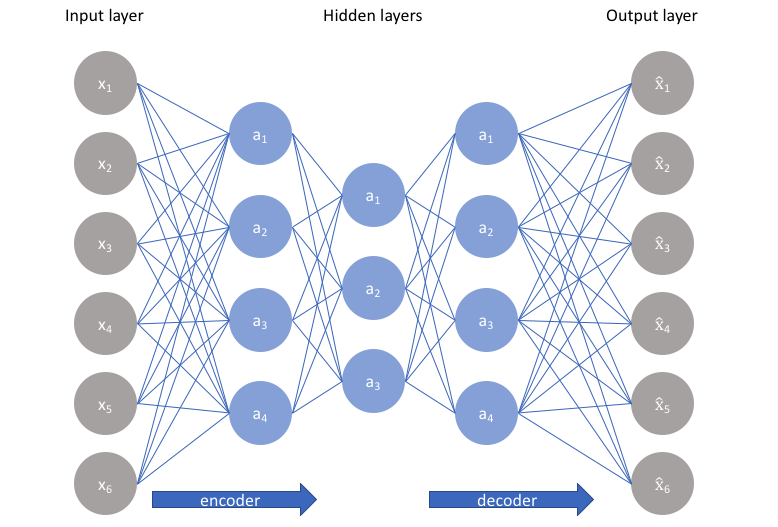
\includegraphics[width=0.5\textwidth]{autoencoder_diagram.png}}
    \end{center}
\end{wrapfigure}

This nonlinear dimension reduction is done by by training a feed forward (FF) neural network to perform the identity mapping, where the network inputs are reproduced at the output layer. The network contains an internal “bottleneck” layer (containing fewer nodes than input or output layers), which forces the network to develop a compact representation of the input data, and two additional hidden layers \autocite{Kramer}. Look to the diagram to the right, for a visualisation of this set-up. 

The particular network that we trained had three hidden layers, as in the diagram. The first, second and third hidden layers are of dimensions $128$, $64$, and $128$, and use the activations tanh, ReLu, and sigmoid, respectively. Training was performed using Adam optimization, MSE loss, and over $400$ epochs. After training, the generated encodings were used to repeat our model fitting procedures for both the binary-relevance KNN and ML-KNN algorithms. 


\subsection{Artificial Neural Networks (Feed-Forward \& Recurrent)}
Classification approaches utilizing different artificial neural networks are also utilized in our project. Inspired by biological nervous systems, neural networks date back to the first half of the $20^{th}$ century with works such as those by McCulloch and Pitts, which could model simple logical operations \autocite{Piccinini}. Since most subsequent work in the following two decades centered around single layer networks, the power of neural networks was restricted to linearly separable problems. This excluded the possibility of learning even simple functions like XOR, which required a second layer \autocite{NNLM}. In the early 1980s, research on neural networks resurged largely due to successful learning algorithms for multi-layer neural networks and are used today for various tasks such as computer vision, associative memory, representation learning, NLP, etc..

\begin{wrapfigure}{l}{0.5\textwidth}
    \begin{center}
        \raisebox{0pt}[\dimexpr\height-0.8\baselineskip\relax]{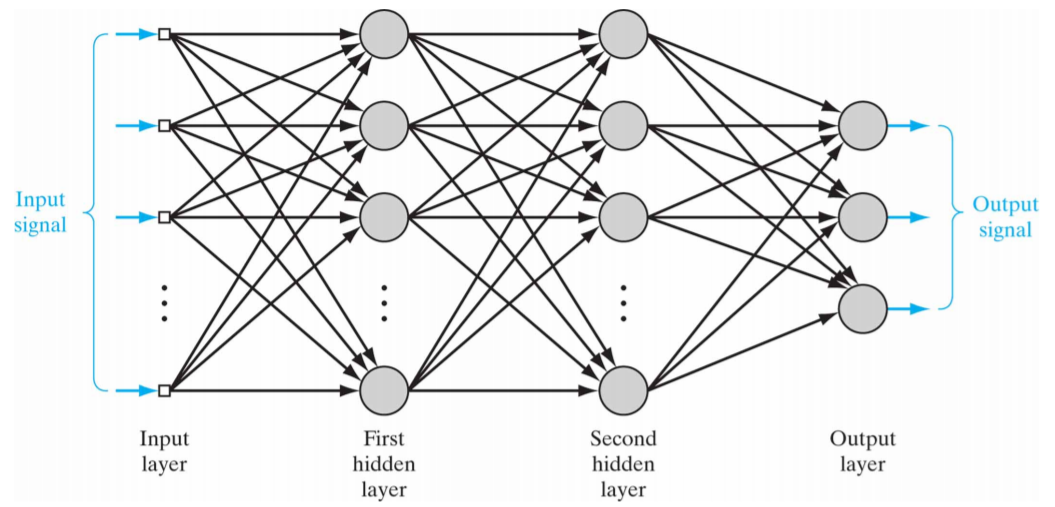
\includegraphics[width=0.5\textwidth]{multilayer_network_Haykin.png}}
    \end{center}
\end{wrapfigure}

For our project, we tried implementing both FF networks and recurrent neural network (RNN) architectures. Perceptrons are the building block for FF networks. A perceptron has an input layer of neurons and an output neuron. Weighted connections exist between every input neuron and the output neuron. A forward pass through the network consists of multiplying the values of the input neurons by the value of their connections' weight, summing and then applying some non-linearity (which we call the activation function). Feed forward networks are typically built by stacking perceptron units vertically and horizontally. All of our FF networks utilize the same architectures; the first hidden layer is of size $32$ with ReLU activation, dropout regularization with drop probability of $0.5$, and an output layer of size $13$ (the number of labels) with sigmoid activations. The FF architectures were trained on $2094$ dimensional tf-idf vectors. 

While FF networks display incredible expressive power, RNNs are a popular adaptation for NLP problems because they are uniquely suited for sequence processing. This is due to their hidden unit connections with shared weights, which allow for information from previous and/or future states to influence the current state. This nice feature also leads to the exacerbation of the "gradient exploding/vanishing" problem during training. Many methods have been proposed to overcome this, one of which is the "gated" architecture we use, known as the Long-Short-Term-Memory (LSTM) architecture. 

On the reduced dataset, all of our RNN models utilize the same bidirectional LSTM architecture. On the full dataset, all of our models utilize the same single-directional LSTM architecture. In both the bidirectional and single-directional LSTM's, we used hidden states of size $16$ followed by a dense output layer with sigmoid activations.The RNNs were trained on padded sequences of integers corresponding to sequences of the processed tokens from the paragraphs; urls, punctuation, and stop words were all removed. 

All of our networks (both FF and RNN) utilize the same optimization algorithm (Adam optimization -- a variant of gradient descent), however, training was performed, using two different loss functions. The standard binary cross entropy loss function was used, in addition, to the more novel BPMLL (back prop for multilabel learning) loss. The BPMLL loss function requires instances to have at least one label. Thus, on the one hand, we trained both cross entropy and BPMLL models on such a reduced dataset in addition to training just cross entropy models on the full dataset. 

The BPMLL loss function aims to leverage correlations between labels by evaluating the error as a function of pairwise errors between labels. Namely, the loss function is given by:

$$
    E = \sum_{i = 1}^m E_i = \sum_{i = 1}^m \frac{1}{|Y_i| |\overline{Y}_i|} \sum_{(k,l) \in Y_i \times \overline{Y}_i} \exp(-(c_k^i - c_l^i))
$$

where $c_j^i = c_j(x_i)$ is the output of the network on $x_i$ on the $j^{th}$ class. The back propagation algorithm is derived in the same manner is for a cross entropy or MSE loss. Details are ommitted here, but can be found in \autocite{bpmll}.
  
\subsection{Threshold Function Learning}

In both of their papers, introducing the BPMLL and ML-KNN algorithms, Zhang \& Zhou also describe a common method for learning threshold functions. Perfect classification, using a constant threshold requires two conditions: (1) Logit values corresponding to labels included in an instance's label set  be separated from logit values corresponding to labels not in an instance's label set. And (2) this separation be around some constant value (usually either $0.5$ or $0$). Learning a threshold function aims to relax the second condition. Namely, we fit a linear regression model to learn threshold values from the logit outputs of our models. For more details, see \autocite{bpmll} \& \autocite{ZhangMulti-labelLazy}. 
\section{Results}

\subsection{ML-KNN Results}

\subsection{Artificial Neural Network Results}

As some instances in the full dataset lack labels,  the 'Reduced Dataset' is created by removing these instances without any labels. The full dataset and reduced dataset are then used to train and validate four networks: Feed Forward network with cross entropy loss(CE FF), Feed Forward network with BPMLL(BPMLL FF),Recurrent neural network with Bidirectional (single directional on full dataset) LSTM and  cross entropy loss(CE RNN), and Recurrent neural network with Bidirectional (single directional on full dataset) LSTM and BPMLL(BPMLL RNN). We also train the neural network using 3 different training rate: 0.01,0.001,0.0001. For each learning rate, the validation set hamming loss is plotted against epochs as shown in figure \ref{fig:example1} and \ref{fig:example2}.

Figure \ref{fig:example1} shows the training history of CE FF and CE RNN using full dataset and constant threshold. From the left and middle sub figures, it can be shown that CE FF can achieve lower hamming loss than CE RNN. For the right sub figure, though the CE FF has higher hamming loss than CE RNN, CE FF seems to have decreasing trend of hamming loss as opposed to the plateau trend of CE RNN at 100 epoch, meaning that it is highly possible that CE FF will have lower hamming loss than CE RNN if the training continues. The effect of learning rate on training is also clear from Figure \ref{fig:example1}: smaller learning rate leads to slower training process. But from figure 1, it is unclear whether  smaller learning rate can reduce the hamming loss finally.

\begin{figure}[!htbp]
\centering 
        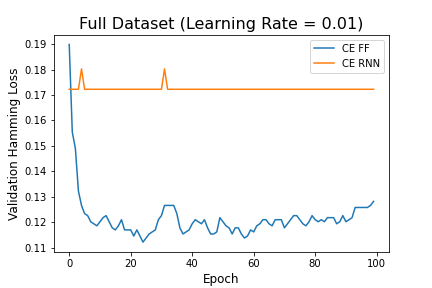
\includegraphics[width=0.32\textwidth,height=4.2cm]{Full_Dataset_Learning_Rate_01.png}
        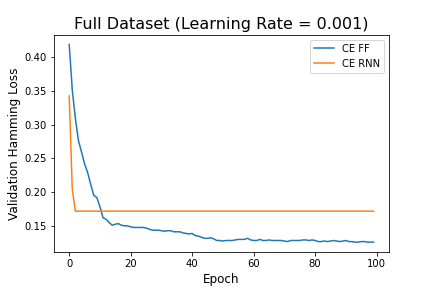
\includegraphics[width=0.32\textwidth,height=4.2cm]{Full_Dataset_Learning_Rate_001.png}
        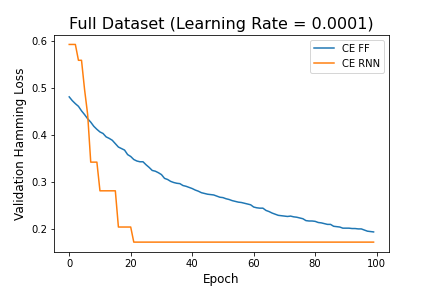
\includegraphics[width=0.32\textwidth,height=4.2cm]{Full_Dataset_Learning_Rate_0001.png}        
\caption[Original image and post processed image]{2 models trained by full dataset}
\label{fig:example1} 
\end{figure}

To compare with constant threshold, table \ref{PVFTD} gives the validation set hamming loss after 100 epochs of training, using a learned threshold function, for each network with 3 different learning rate. No significant improvement in hamming loss has been observed for both 2 networks after learned threshold function is used.

In contrast with constant constant thresholds, this time CE FF seems to have higher hamming loss than CE RNN for all 3 learning rate. It also seems that the learning rate of 0.001 has the lowest hamming loss.

 \begin{longtable}[c]{| p{.27\textwidth} | p{.27\textwidth} |p{.27\textwidth} |}
\hline
        Learning Rate  & CE FF & CE RNN  \\
        \hline
         0.01 & 0.3020833333 & 0.2379807692 \\
        \hline
         0.001 & 0.17868589740 & 0.1730769231 \\
        \hline
         0.0001 & 0.2115384615 & 0.1770833333 \\
        \hline        
\caption{Hamming Loss with Threshold Function Learning}
\label{PVFTD}
\end{longtable}

All the 4 models are trained with the reduced dataset using constant threshold and the results are shown in figure \ref{fig:example2}. Similar to the full dataset case, RNN in general has higher hamming loss than Feed-Forward for learning rate of 0.01 and 0.001. The same conclusion seems to hold for learning rate of 0.0001 if training epoches increase. 

From the right and middle sub figures, for both RNN and Feed-Forward network, the hamming loss is quite close between BPMLL and cross entropy. In fact, the left sub figure shows BPMLL has higher hamming loss than cross entropy for both RNN and Feed-Forward network.

Also, smaller learning rate needs more training epoches for finale convergence. 

\begin{figure}[!htbp]
\centering 
        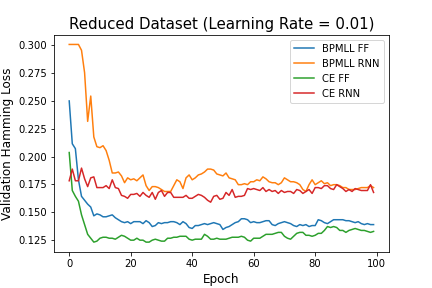
\includegraphics[width=0.32\textwidth,height=4.2cm]{Reduced_Dataset_Learning_Rate_01.png}
        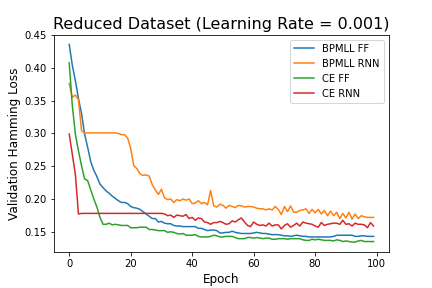
\includegraphics[width=0.32\textwidth,height=4.2cm]{Reduced_Dataset_Learning_Rate_001.png}
        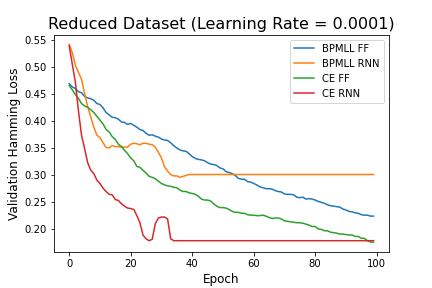
\includegraphics[width=0.32\textwidth,height=4.2cm]{Reduced_Dataset_Learning_Rate_0001.png}        
\caption[Original image and post processed image]{4 models trained by reduced dataset}
\label{fig:example2} 
\end{figure}

Similarly, as shown in Table \ref{PVFTT}, the 4 models are also trained with Threshold Function Learning, but the hamming loss is not reduced for all 4 models. Also, no clear winner among 4 models is observed. 
 \begin{longtable}[c]{| p{.17\textwidth} | p{.17\textwidth} |p{.17\textwidth} |p{.17\textwidth} |p{.17\textwidth} |}
\hline
        Learning Rate  & CE FF & BPMLL FF &CE RNN &BPMLL RNN  \\
        \hline
         0.01 & 0.1520979021 & 0.145979021 & 0.2447552448 & 0.2194055944\\
        \hline
         0.001 & 0.1853146853 & 0.2578671329 & 0.1791958042 & 0.20454545\\
        \hline
         0.0001 & 0.2071678322 & 0.1844405594 & 0.1896853147 & 0.2132867133\\
        \hline        
\caption{Hamming Loss with Threshold Function Learning}
\label{PVFTT}
\end{longtable}
\section{Discussion \& Conclusions}

\newpage
\printbibliography

\end{document}

